\section{Relative Homologie einer Chirurgie}
    \begin{theorem}
        F\"ur \(i\leq j-1\) gelten
        \[H_k(\mathcal{M}^{\prime},\mathcal{M}_0)\cong\begin{cases}
            \mathbb{Z} & k\in\{0,i+1\}\\
            0 & 1<k<i+1
        \end{cases}\]
        und 
        \[H_k(\mathcal{M},\mathcal{M}_0)\cong\begin{cases}
            \mathbb{Z} & k\in\{0,j+1\}\\
            0 & 1<k<j+1
        \end{cases}\,.\]
        Erzeuger der \(\mathbb{Z}\)-Anteile in Dimension \(i+1\) und \(j+1\) sind der Kern \((\mathbb{D}^{i+1},\mathbb{S}^i)\) und der Kokern \((\mathbb{D}^{j+1},\mathbb{S}^j)\).
    \end{theorem}
    \begin{proof}
        Die lange exakte Folge des Tripels \((\mathbb{D}^{i+1}\times\mathbb{D}^{j+1},\mathbb{D}^{i+1}\times\mathbb{S}^j,\mathbb{S}^i\times\mathbb{S}^j)\) ist von der Form
        \begin{center}
            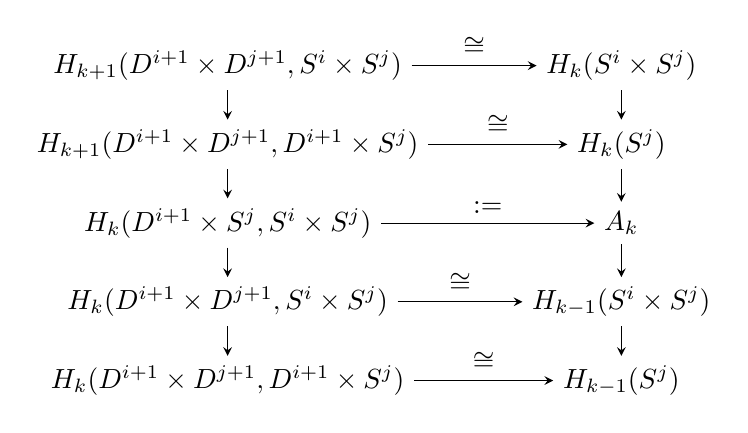
\begin{tikzpicture}
                \draw
                (-3, 1) node (A) {\(H_{k+1}(\mathbb{D}^{i+1}\times\mathbb{D}^{j+1},\mathbb{S}^i\times\mathbb{S}^j)\)}
                (-3, 0) node (B) {\(H_{k+1}(\mathbb{D}^{i+1}\times\mathbb{D}^{j+1},\mathbb{D}^{i+1}\times\mathbb{S}^j)\)}
                (-3, -1) node (C) {\(H_k(\mathbb{D}^{i+1}\times\mathbb{S}^j,\mathbb{S}^i\times\mathbb{S}^j)\)}
                (-3, -2) node (D) {\(H_k(\mathbb{D}^{i+1}\times\mathbb{D}^{j+1},\mathbb{S}^i\times\mathbb{S}^j)\)}
                (-3, -3) node (E) {\(H_k(\mathbb{D}^{i+1}\times\mathbb{D}^{j+1},\mathbb{D}^{i+1}\times\mathbb{S}^j)\)}
                
                (2, 1) node (F) {\(H_k(\mathbb{S}^i\times\mathbb{S}^j)\)}
                (2, 0) node (G) {\(H_k(\mathbb{S}^j)\)}
                (2, -1) node (H) {\(A_k\)}
                (2, -2) node (I) {\(H_{k-1}(\mathbb{S}^i\times\mathbb{S}^j)\)}
                (2, -3) node (J) {\(H_{k-1}(\mathbb{S}^j)\)}
    
                (A) edge [-stealth] (B)
                (B) edge [-stealth] (C)
                (C) edge [-stealth] (D)
                (D) edge [-stealth] (E)
                
                (F) edge [-stealth] (G)
                (G) edge [-stealth] (H)
                (H) edge [-stealth] (I)
                (I) edge [-stealth] (J)
                
                (A) edge [-stealth] node [above] {\(\cong\)} (F)
                (B) edge [-stealth] node [above] {\(\cong\)} (G)
                (C) edge [-stealth] node [above] {\(:=\)} (H)
                (D) edge [-stealth] node [above] {\(\cong\)} (I)
                (E) edge [-stealth] node [above] {\(\cong\)} (J)
                ;
            \end{tikzpicture}
        \end{center}
        Ebenso ist die lange exakte Folge f\"ur \((\mathbb{D}^{i+1}\times\mathbb{D}^{j+1},\mathbb{S}^i\times\mathbb{D}^{j+1},\mathbb{S}^i\times\mathbb{S}^j)\) von der Form
        \[H_k(\mathbb{S}^i\times\mathbb{S}^j)\to H_k(\mathbb{S}^i)\to B_k\to H_{k-1}(\mathbb{S}^i\times\mathbb{S}^j)\to H_{k-1}(\mathbb{S}^i)\,.\]
        Aus \(k\notin\{j,j+1\}\) folgt direkt 
        \begin{equation}
            A_k:=H_k(\mathbb{D}^{i+1}\times\mathbb{S}^j,\mathbb{S}^i\times\mathbb{S}^j)\cong H_{k-1}(\mathbb{S}^i\times\mathbb{S}^j)\,,
        \end{equation}
        aus \(k\notin\{i,i+1\}\)
        \begin{equation}
            B_k:=H_k(\mathbb{S}^i\times\mathbb{D}^{j+1},\mathbb{S}^i\times\mathbb{S}^j)\cong H_{k-1}(\mathbb{S}^i\times\mathbb{S}^j)\,.
        \end{equation}
        Dies impliziert \(A_k=0\) f\"ur \(1<k<j\) und \(B_k=0\) f\"ur \(1<k<i\). Interessant ist nun das Verhalten von \(\{i,i+1\}\cap\{j,j+1\}\). Es gibt drei F\"alle: \(i=j-1\), \(i=j\) und \(i=j+1\). Hierbei \"ubernehmen \(i\) und \(j\) f\"ur \(A_i\) und \(B_i\) duale Stellungen, sodass in den langen exakten Folgen von oben essenziell drei F\"alle eintreten k\"onnen.
        
        \subsubsection{Fall \(1\)}
            Es ergeben sich die exakten Folgen
            \[0\to A_{i+2}\rightarrowtail\mathbb{Z}\mathop{\longrightarrow}^{\mathbbm{1}}\mathbb{Z}\to A_{i+1}\twoheadrightarrow\mathbb{Z}\to0\quad\text{f\"ur}\quad i=j+1\,,\]
            \[0\to B_{j+2}\rightarrowtail\mathbb{Z}\mathop{\longrightarrow}^{\mathbbm{1}}\mathbb{Z}\to B_{j+1}\twoheadrightarrow\mathbb{Z}\to0\quad\text{f\"ur}\quad j=i+1\,,\]
            also folgt \(A_{i+2}\cong\ker\mathbbm{1}=0\). Da die Identit\"at surjektiv ist, ist der Morphismus \(\mathbb{Z}\to A_{i+1}\) gleich null, also folgt \(A_{i+1}\cong\mathbb{Z}\). Komplett analog folgen \(B_{j+2}=0\) und \(B_{j+1}\cong\mathbb{Z}\).
            
        \subsubsection{Fall \(2\)}
            Sei \(i=j\). Dann ergeben sich die exakten Folgen
            \[0\to A_{i+1}\rightarrowtail\mathbb{Z}\oplus\mathbb{Z}\mathop{\longrightarrow}^{\pi_2}\mathbb{Z}\twoheadrightarrow A_i\to0\]
            \[0\to B_{j+1}\rightarrowtail\mathbb{Z}\oplus\mathbb{Z}\mathop{\longrightarrow}^{\pi_1}\mathbb{Z}\twoheadrightarrow B_j\to0\]
            Der mittlere Homomorphismus ist surjektiv, also gelten
            \[A_{i+1}\cong\ker\pi_2=\mathbb{Z}\quad\text{und}\quad A_i\cong\operatorname{coker}\pi_2=0\,,\]
            und analog \(B_{j+1}\cong\mathbb{Z}\) und \(B_j=0\).
            
        \subsubsection{Fall \(3\)}
            Es ergeben sich die exakten Folgen
            \[0\to A_{i+1}\mathop{\to}^{\sim}\mathbb{Z}\to0\to A_i\rightarrowtail\mathbb{Z}\mathop{\longrightarrow}^{\mathbbm{1}}\mathbb{Z}\twoheadrightarrow A_{i-1}\to0\quad\text{f\"ur}\quad i=j-1\,.\]
            \[0\to B_{j+1}\mathop{\to}^{\sim}\mathbb{Z}\to0\to B_j\rightarrowtail\mathbb{Z}\mathop{\longrightarrow}^{\mathbbm{1}}\mathbb{Z}\twoheadrightarrow B_{j-1}\to0\quad\text{f\"ur}\quad j=i-1\,.\]
            Direkt folgen \(A_{i+1}\cong\mathbb{Z}\) und \(B_{j+1}\cong\mathbb{Z}\), sowie
            \[A_i\cong B_j\cong\ker\mathbbm{1}=0\quad\text{und}\quad A_{i-1}\cong B_{j-1}\cong\operatorname{coker}\mathbbm{1}=0\,.\]
    \end{proof}